\documentclass[conference]{IEEEtran}

\usepackage{cite}
\usepackage[pdftex]{graphicx}
\usepackage{amsmath}
\usepackage{array}
\usepackage[caption=false,font=footnotesize]{subfig}
\usepackage{fixltx2e}
\usepackage{stfloats}
%\usepackage{dblfloatfix}
\usepackage{color}

\interdisplaylinepenalty=2500

\hyphenation{op-tical net-works semi-conduc-tor}

\begin{document}

\title{Arabic Manuscript Author Verification Using\\ 
Deep Convolutional Networks}

\author{\IEEEauthorblockN{Andrei Boiarov\IEEEauthorrefmark{1},
Alexander Senov\IEEEauthorrefmark{1} and
Alexander Knysh\IEEEauthorrefmark{2}\IEEEauthorrefmark{3}}
\IEEEauthorblockA{\IEEEauthorrefmark{1}Faculty of Mathematics and Mechanics\\
Saint Petersburg State University,
Saint Petersburg, Russia\\ Email: andrei.boiarov@gmail.com, alexander.senov@gmail.com}
\IEEEauthorblockA{\IEEEauthorrefmark{2}Department of Near Eastern Studies\\
University of Michigan, Ann Arbor, Michigan, USA}
\IEEEauthorblockA{\IEEEauthorrefmark{3}Research Laboratory for Analysis and Modeling of Social Processes\\
Saint Petersburg State University, Saint Petersburg, Russia\\
Email: alknysh@umich.edu}}

\maketitle

\begin{abstract}
In this paper, we propose an automatic method for manuscript author verification based on an analysis of consecutive patches extracted from an image. The classification algorithm uses a deep convolutional network with two types of patch extraction: one based on connected components and the other based on usage of a fixed-size sliding window. We apply this method to verify the authorship of the Arabic manuscript entitled \textit{al-Khitat} attributed to the hand of the renowned  medieval Arab historian al-Maqrizi. Using appropriately collected ground-truth labeled data for convolutional network training purpose, our method has demonstrated promising results when applied to previously unseen manuscripts.
\end{abstract}

\IEEEpeerreviewmaketitle

\section{Introduction}
\label{sec:introduction}
The problem of manuscript author verification is quite important nowadays. Since manual verification has a subjectivity drawback, the solution requires objective automatic methods. The present study was motivated by the recent discovery by Dr. Noah Gardiner of the holograph (autograph) copy of the third volume of al-Maqrizi's famous ``Description of Egypt'' in the Library of the University of Michigan \cite{Noah}. The full title of the manuscript is ``The Book of Admonitions and Lessons in the Catalogue of Territorial Divisions and Historical Monuments'', usually cited by its abbreviated Arabic title as \textit{al-Khitat}. The manuscript was complited shortly after 831 A.H. (1427 C.E.) by the celebrated Egyptian historian Taqi al-Din Ahmad Ibn Ali al-Maqrizi (d. 845/1442). In his paper, Dr. Gardiner made the assumption that it might be a draft copy of the work. He then sent images of the codex to Prof. Frederic Bauden of the University of Liege, the author of numerous articles on al-Maqrizi autographs. Bauden identified it as the fair copy (the author's final version) of the third volume of \textit{al-Khitat}, and thus the only fair copy of any volume of \textit{al-Khitat} to have been found thus far.

Given the importance of this discovery for the history of science (al-Maqrizi's \textit{al-Khitat} is one of the earliest descriptions of the topography of Cairo and ancient Egyptian monuments in its environs as well as Alexandria), the authors of this paper decided to verify Dr. Gardiner's and Prof. Bauden's findings using method based on deep convolutional networks.

Previously used methods for author verification of Arabic manuscripts and for related fields were focused on developing various types of features that can be obtained from a manuscript picture. These features are then used to learn a classification model. Here are some of the approaches: textural, allographic features and clustering methods \cite{MBulacu}, \cite{MBulacu1}; contour-based, oriented basic image, K-SIFT features and SVM \cite{DFecker}, texture-related and structure-related features \cite{Salvador}, TF/IDF and clustering algorithms \cite{Dunn}. In this paper, we present a novel approach based on learning of deep hierarchical structure of features from the row image. This method belongs to the class of the deep learning algorithms \cite{DL} and uses convolutional network \cite{CNN} for feature extraction and prediction. Deep learning methods were used in tasks from nearby fields, for example \cite{DL_Arabic_1}, \cite{DL_Arabic_2}. Our approach was designed for the particular purpose of al-Maqriz's authorship verification. To solve this problem, the methods described above need to be adapted, so it was decided to apply instead a new promising deep learning approach. Since year deep convolution networks \cite{Alexnet} have become the state of the art in many areas of computer vision: object recognition, face identification, optical character recognition, object detection, etc \cite{DL}. Deep learning approach is based on using artificial neural networks with a large number of layers which allows to train deep hierarchical representation of data. This representation in many cases works better then handmade features \cite{DL}, \cite{Alexnet}, \cite{Googlenet}. Moreover deep networks are not saturated with an increasing amounts of data thus they have better generalization ability then traditional ``shallow'' methods like logistic regeression or SVM \cite{DL}.   

The paper is organized as follows. In Section~\ref{sec:the_data}, a description of the data set used in experiments is given. Section~\ref{sec:the_method} contains presentation of our methodology of patches from image extraction, training deep convolution networks and making decision regarding of manuscript author. In Section~\ref{sec:results_and_description}, we present the results of our experiments.
%\pagebreak
	

\begin{figure*}[!t]
	\center
  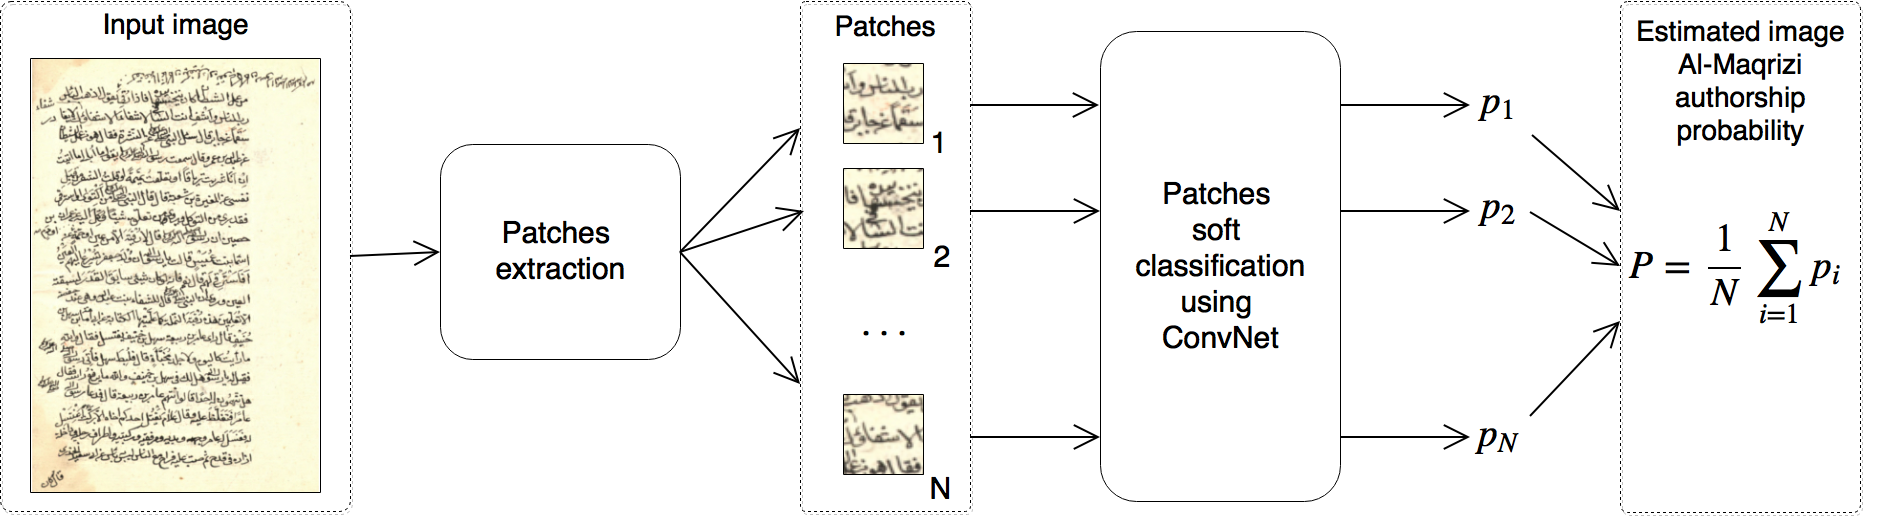
\includegraphics[width=0.9\textwidth]{figures/Al-Maqrizi_classification_pipeline.png}
  \caption{al-Maqrizi authorship classification pipeline}
  \label{fig:pipeline}
\end{figure*}	
	
\section{Data Set}
\label{sec:the_data}

Solving the problem of al-Maqrizi's authorship requires training and test data sets. 
We consider a single page of the manuscript as one data unit.
As a one unique data element we consider single page of manuscript. The data set consists of two sets of manuscript materials.
\begin{itemize}
	\item Two holographs by al-Maqrizi verified by Prof. Bauden will serve as a positive example.
	\item Eight manuscripts not written by al-Maqrizi's hand  (taken from the University of Michigan Hatcher Library Special Collections) are considered to be a negative example. These manuscripts were selected so that the date and place of writing of each of them would be close to those of al-Maqrizi's  \textit{al-Khitat}, namely, the 14th and 15th centuries, in Egypt and Syria.
\end{itemize}

To enhance the robustness of the learning process the data obtained were divided into training and test sets:
\begin{itemize}
	\item Training set: 1 al-Maqrizi's manuscript consisting of 26 pages and 5 non-al-Maqrizi's manuscripts each of which consists of 7 pages.
	\item Test set: 1 al-Maqrizi's manuscript consisting of 14 pages and 3 non-al-Maqrizi's manuscripts each of which consists of 7 pages. Authors of these 3 manuscripts differ from authors of 5 negative examples in the training set.   
\end{itemize}

Two examples from the training set is illustrated by Figure~\ref{fig:train_examp}. 

It is important to note that we split our data set by the factor of the manuscript author. When the algorithm is learning on the training set, it cannot see the authors in the test set. Thus, we apply our method to infer general properties al-Maqrizi's handwriting not specific to a particular manuscript. The number of non-al-Maqrizi's documents is chosen in such way that positive and negative classes in training and test sets are roughly balanced.

The goal of this study is to verify the authorship of the \textit{al-Khitat} manuscript that consists of 32 pages.

\begin{figure}[!t]
	\centering
  	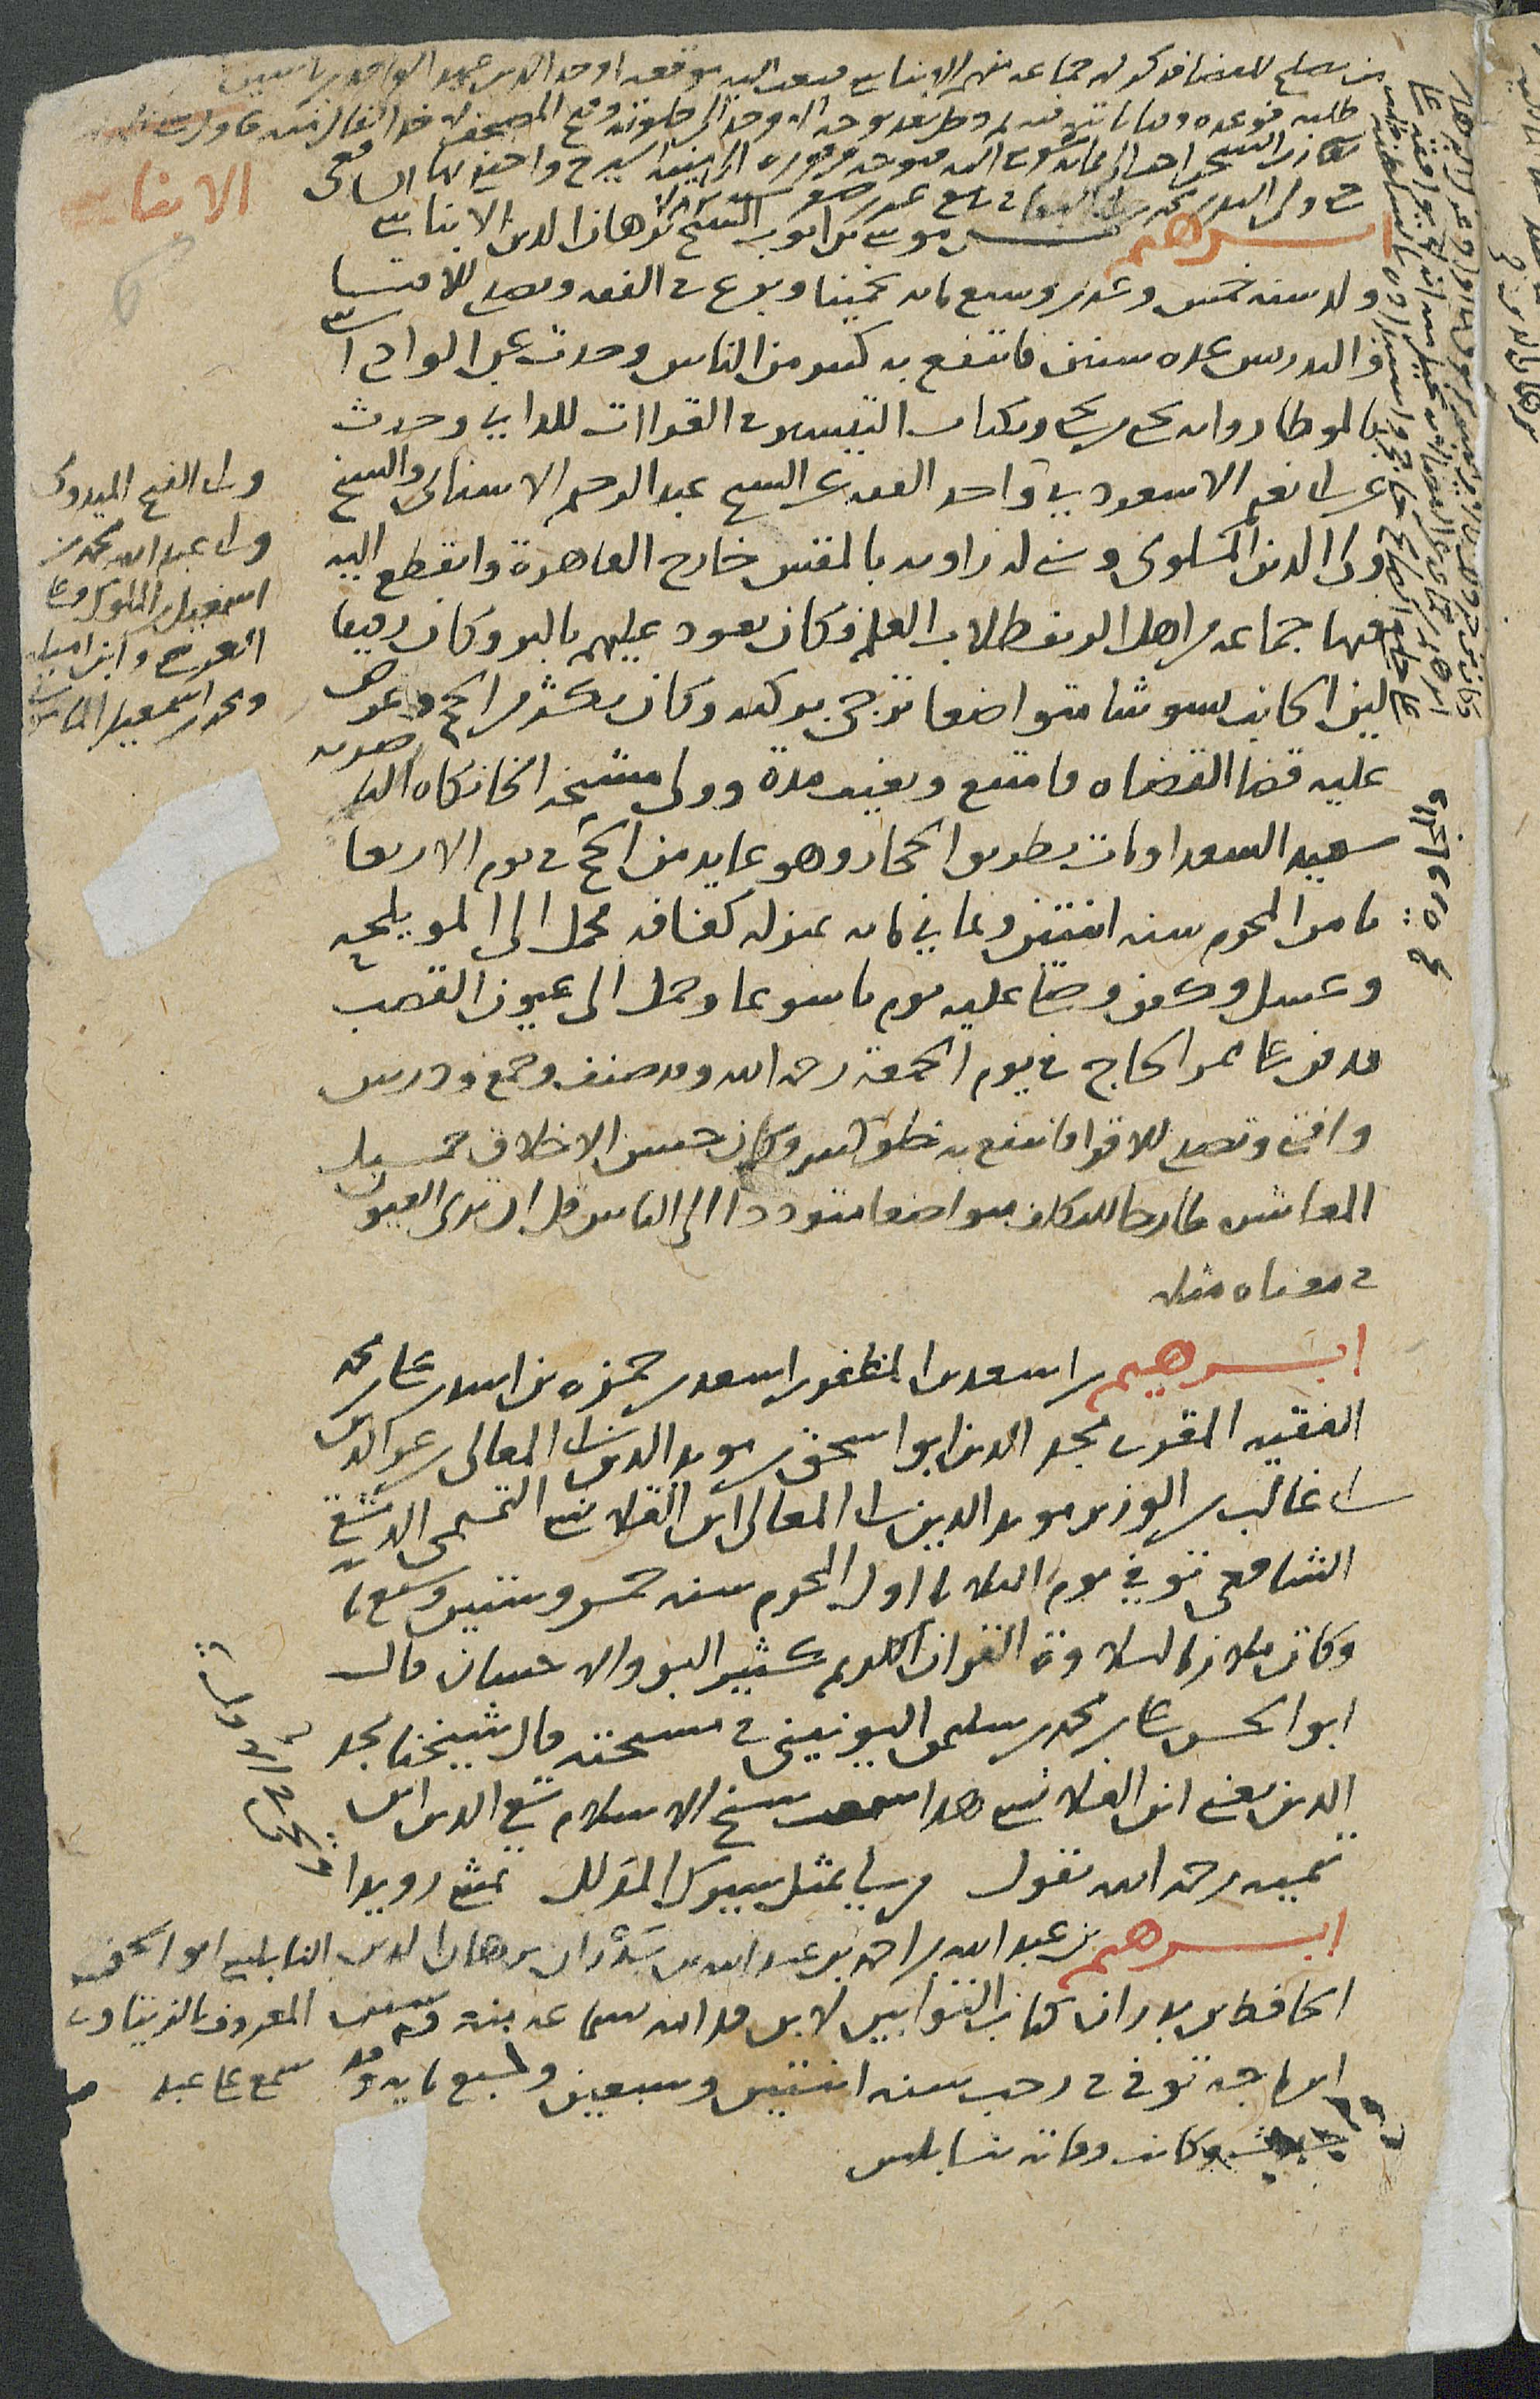
\includegraphics[width=0.45\linewidth]{figures/Ms-orient-A-01771_017.jpg}
  	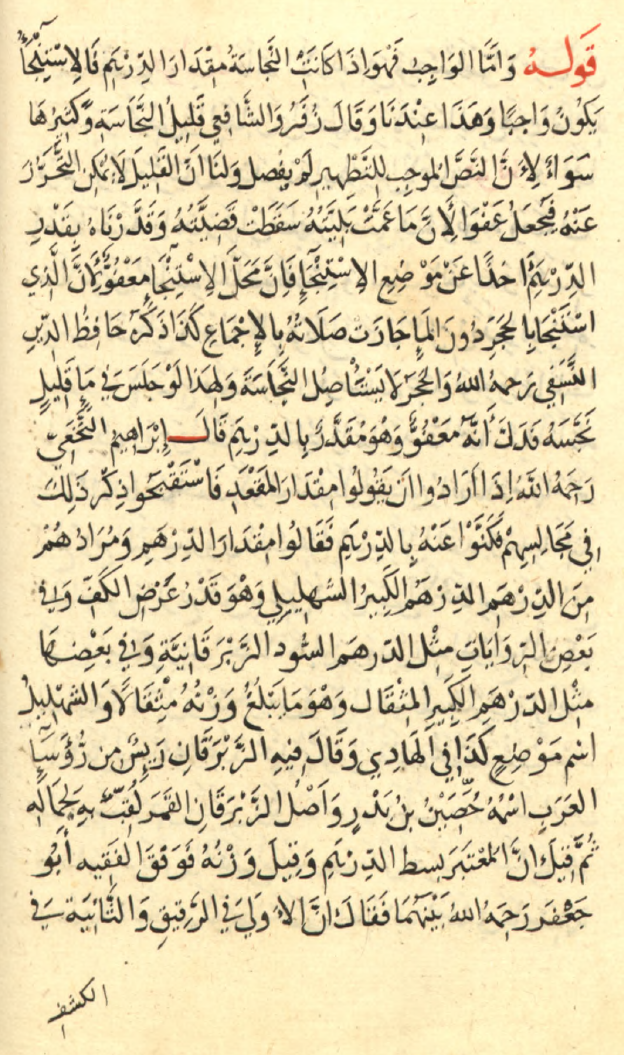
\includegraphics[width=0.415\linewidth]{figures/5_test_1.png}
  	\caption{Examples of al-Maqrizi (left) and not al-Maqrizi (manuscript from Cairo, 1466 C.E.) (right) holographs from training set}
	\label{fig:train_examp}
\end{figure}

%\pagebreak

\section{Method}
\label{sec:the_method}

We consider author verification as a binary classification problem: positive class designated as 1 consists of images that belong to al-Maqrizi's hand and negative class designated as 0 consist of images by the hand of a different author. In this context our goal is to build a classification pipeline able to estimate the probability (\textit{soft} classification) that a given image belongs to the $1$ (al-Maqrizi) class. Thus, the perfect classifier should return 1 for all al-Maqrizi's images and 0 for all non-al-Maqrizi's images. The entire proposed classification pipeline for al-Maqrizi authorship verification illustrated in Figure~\ref{fig:pipeline} consists of the following steps:

\begin{enumerate}
	\item Image preprocessing.
	\item Extracting patches from candidate image.
	\item Soft classification of patches using convolution network.
	\item Averaging predicted patches probabilities to produce an overall candidate image of the probability of al-Maqrizi's authorship.
\end{enumerate}

Each of these steps are described in the following sections.	


\subsection{Image preprocessing}
Image preprocessing was done to bring all images to a relatively same size and scale by performing the following steps:
\begin{enumerate}
	\item Removing part of image within the text bounding box.
	\item Resizing the resulted image to fixed resolution $(700\times 500)$.
\end{enumerate}
These steps are reasonable enough, since all images from our data set have approximately equal number of text lines, relative font size and text bounding box aspect ratio. Thus, by removing a blank margin from image and resizing it to fixed size we make our classification problem simplier since images become less diverse. 

Note: since this step is done only to unify our images data set we did not include it into the pipeline in Figure~\ref{fig:pipeline}.

\subsection{Patches extraction}
Patches extraction is a process of breaking given image into a set of potentially overlapping sub-images called patches. The basic idea is that a patch should represent a small but yet meaningful part of an image for the purpose of authorship verification. On the one hand, patches should be as small as possible to reduce the dimension of input vector for classification, but, on the other hand, patches still should contain enough information for successful authorship verification.  

We use two alternative methods for patches extraction. Both of them are described below.

\textit{Sliding window based method:}
This method uses sliding window of the size $80\times 80$ pixels, a stride of size $20$ pixels and operates in the following way:
\begin{enumerate}
  \setcounter{enumi}{-1}
	\item Sliding window moved to the top left conner of the image.
	\item Patch extracted from the current window position.
	\item Sliding window shifts to the right on the stride size, if possible. Otherwise it is moved to the leftmost position and shifted down on the stride size.
	\item Goto 1.
\end{enumerate} 
Figure~\ref{fig:patches_example_sliding_window} demonstrates an example of the resultant patch.

\textit{Connected components-based method:}
This method attempts to extract patches containing one or several symbols on the same text line by utilizing the idea of connected components. Its general scheme is described below.
\begin{enumerate}
	\item First, the input image is binarized using Otsu's filter~\cite{otsu1975threshold}. After this step images consist of only 1's (symbols) and 0's (blank space).
	\item Then, connected components of 1's are extracted from a binarized image using the algorithm from~\cite{fiorio1996connected_components}. 
	\item The connected components that are too small, too big or too stretched are filtered out using several empirical rules, e.g.: major axis to minor axis ratio less then $10$, minimum minor axis length greater then $3$ pixels, maximum major axis length less then $220$ pixels and  minimum major axis length greater then 5.
	\item Points of connected components' centers are clustered using DBSCAN clustering algorithm~\cite{ester1996dbscan,GranVolk} with the following parameters: epsilon = 0.5 and minimum number of points to form a dense cluster = 10. Thereupon connected components corresponding to the points which do not fall in any cluster are labelled as outliers and filtered out.
	\item Finally, the remaining connected components bounding boxes are extracted from the source image and resized to $28\times 28$ pixels size.
\end{enumerate}

Example of the connected components based patches shown on Figure~\ref{fig:patches_example_connected_components}. 

As one can see, connected components-based patches usually consist of one or several letters thus providing a high robustness for a different image scale and size in contrast to the fixed-size sliding window patches (since all images have been preprocessed this feature is not important in our case). However, sliding-window patches contain much more information: several symbols from multiple lines --- a very important feature for authorship verification.
%
%\begin{figure}[!b]
%    \centering
%    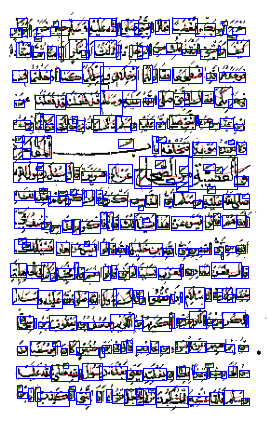
\includegraphics[width=0.2\textwidth]{figures/patches_example_connected_components.png}	 
%	\hfill    
%    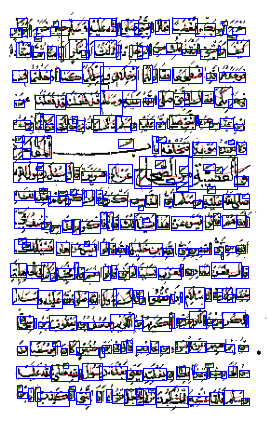
\includegraphics[width=0.2\textwidth]{figures/patches_example_connected_components.png} 
%%    \caption{2 Figures side by side}%
%    \label{fig:example}%
%\end{figure}

%\begin{figure}
%	\centering
%	\begin{minipage}{0.1\textwidth}
%	\centering
%	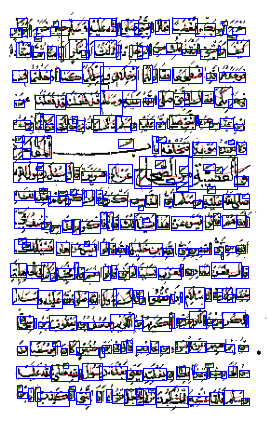
\includegraphics{figures/patches_example_connected_components.png}
%	\caption{first figure}
%	\end{minipage}
%	\hfill
%	\begin{minipage}{0.1\textwidth}
%	\centering
%	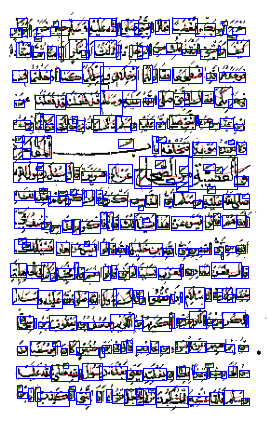
\includegraphics{figures/patches_example_connected_components.png}
%	\caption{second figure}
%	\end{minipage}
%\end{figure}

\begin{figure}[!t]
\centering
\begin{minipage}{.45\linewidth}
	\centering
  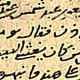
\includegraphics[height=.7\linewidth]{figures/3.png}
  \caption{Sliding window patch example}
  \label{fig:patches_example_sliding_window}
\end{minipage}
\hspace{.05\linewidth}
\begin{minipage}{.45\linewidth}
	\centering
  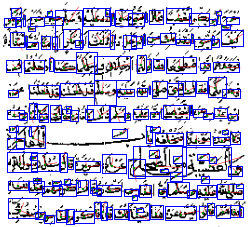
\includegraphics[height=.7\linewidth]{figures/patches_example_connected_components_part.png}
  \caption{Connected components patches example}
  \label{fig:patches_example_connected_components}
\end{minipage}
\end{figure}

%\begin{figure}
%	\centering
%	\subcaptionbox{A cat\label{cat}}
%	[.4\linewidth]{\includegraphics{figures/patches_example_connected components.png}}%
%	\subcaptionbox{An elephant\label{elephant}}
%	[.4\linewidth]{\includegraphics{figures/patches_example_connected components.png}}
%	\caption{Two animals}\label{animals}
%\end{figure}

\subsection{Deep convolution network}

Denote $x_i$ as the $i$-th patch obtained from an image in the previous step and $y_i$ as binary label. Then for predicting the probability
\begin{equation*}
	p_i = P(y_i | x_i)
\end{equation*}
that the current patch belongs to al-Maqrizi's hand we need to train a discriminative model. As a robust and powerful classification algorithm deep convolution networks \cite{DL}, \cite{CNN} are chosen. During experiments various architectures of networks were tested, whereupon the ones that showed best results were selected.

In a case of the sliding window patches we apply AlexNet type of network \cite{Alexnet}. Its architecture and layers parameters is described in Table~\ref{alexnet_tab}. This table contains the following columns: layer type, patch size and stride parameters for convolutional and pooling layers, as well as the number of layer output neurons.% Network architecture is illustrated on Figure~\ref{fig:alexnet}. 
\begin{table}[!b]
\centering
\caption{Sliding window patch convolution network}
\label{alexnet_tab}
\begin{tabular}{|l|p{1.3cm}|p{1.3cm}|}
\hline
\textbf{layer type} & \textbf{patch size/ stride} & \textbf{output number}  \\
\hline
convolution & 11 / 4 & 96 \\
\hline
local response norm & & 96 \\
\hline
max pool & 3 / 2 & 96 \\
\hline
convolution & 5 / 1 & 256 \\
\hline
local response norm & & 256 \\
\hline
max pool & 3 / 2 & 256 \\
\hline
convolution & 3 / 1 & 384 \\
\hline
convolution & 3 / 1 & 384 \\
\hline
convolution & 3 / 1 & 256 \\
\hline
max pool & 3 / 2 & 256 \\
\hline
fully connected & & 4096 \\
\hline
dropout (50 \%) & & 4096 \\
\hline
fully connected & & 4096 \\
\hline
dropout (50 \%) & & 4096 \\
\hline
fully connected & & 2 \\
\hline
softmax & & 2 \\
\hline
\end{tabular}
\end{table}

%\begin{figure}[!b]
%	\centering
%  	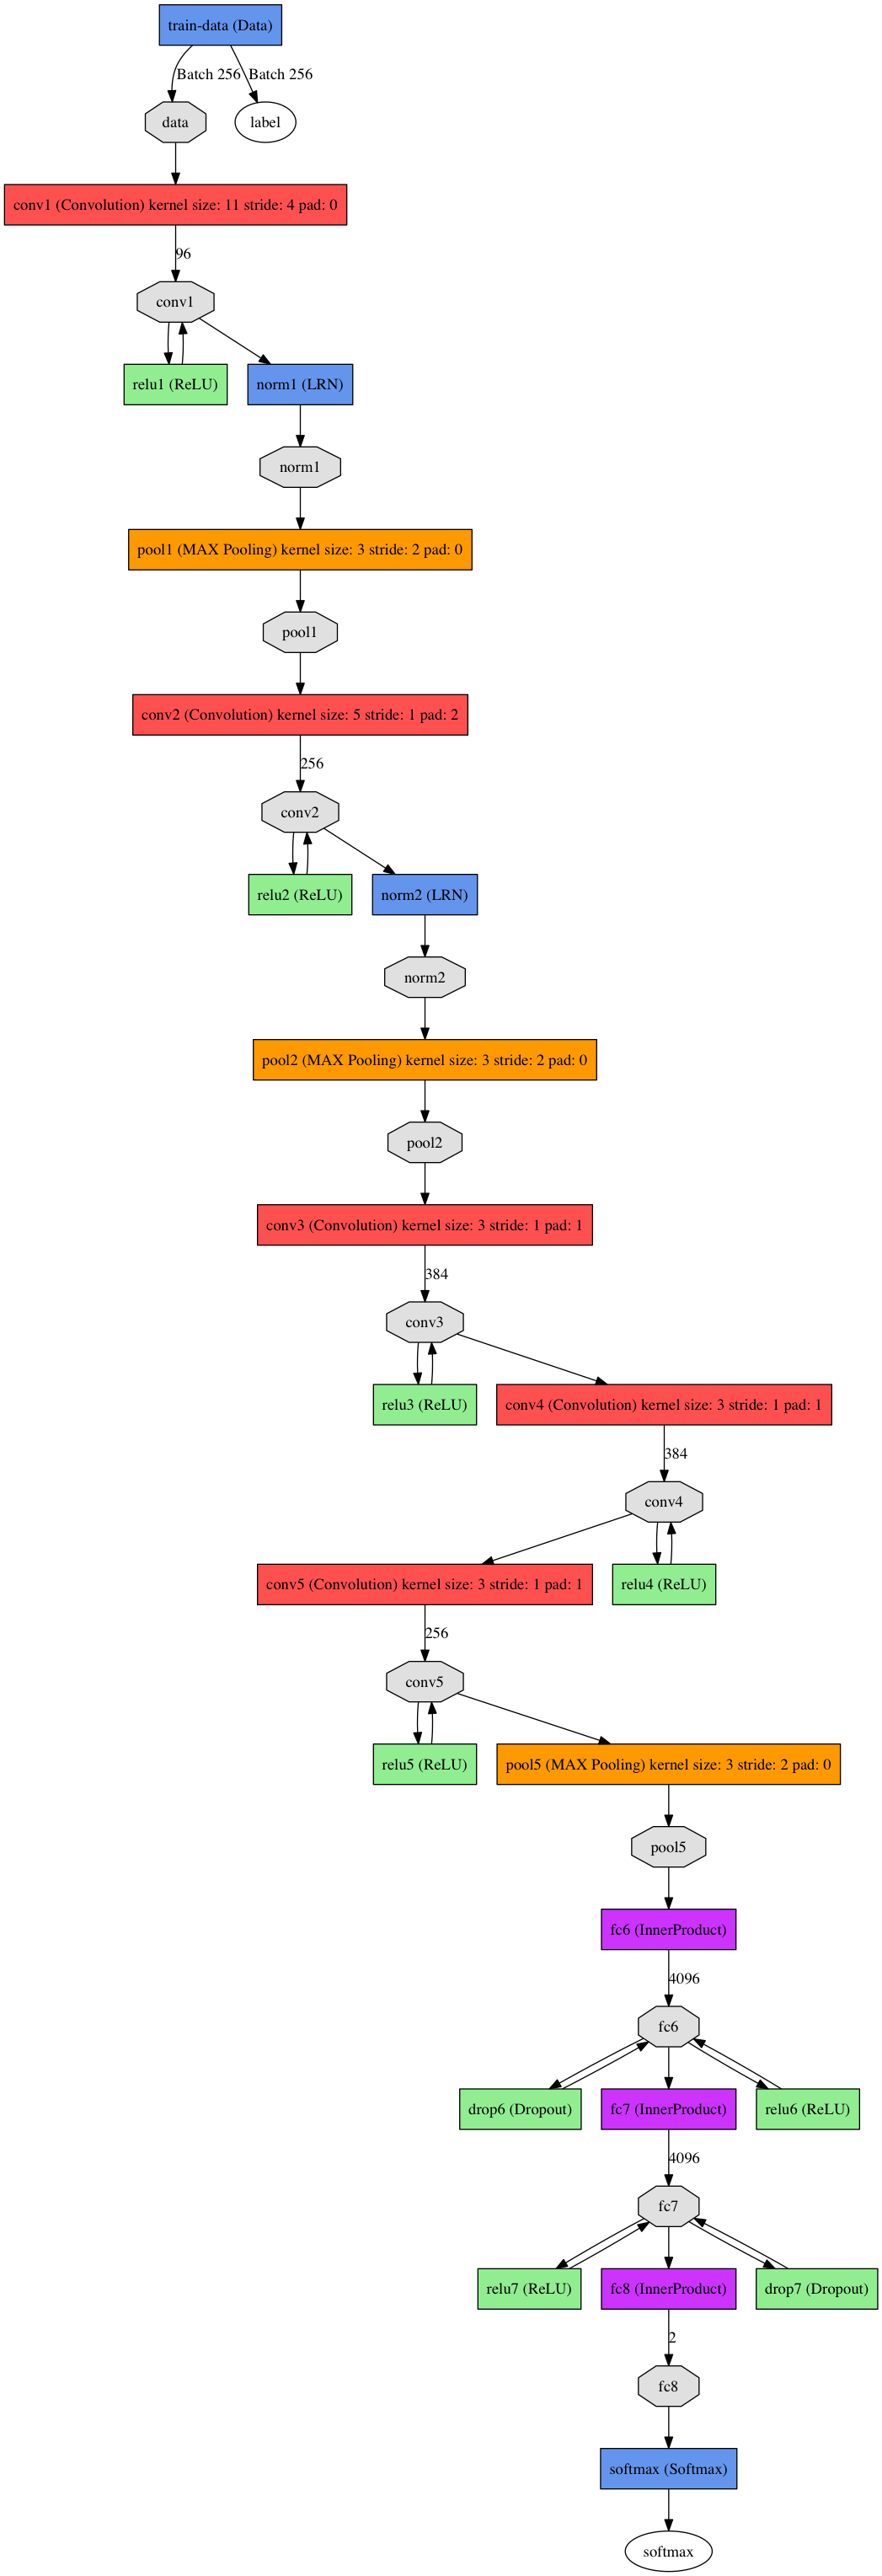
\includegraphics[width=0.85\linewidth]{figures/alexnet.png}
%	\caption{Sliding window patch convolution network architecture}
%  	\label{fig:alexnet}
%\end{figure}

As an input network takes $80\times80$ RGB image. All activation functions in convolution and fully connected layers are rectified linear units (ReLU): $f(x)=\max(0, x)$. This deep network is trained by stochastic gradient descent method with Nesterov momentum, the initial learning rate is $0.01$ and its decrease policy is step down. 

With the connected components patches we use GoogLeNet type of deep convolutional network \cite{Googlenet}. Its architecture and layers parameters are shown in Table~\ref{googlenet_tab}.
\begin{table}[!t]
\centering
\caption{Connected components patch convolution network}
\label{googlenet_tab}
\begin{tabular}{|l|p{1.3cm}|p{1.3cm}|}
\hline
\textbf{layer type} & \textbf{patch size/ stride} & \textbf{output number}  \\
\hline
convolution & 7 / 2 & 64 \\
\hline
max pool & 3 / 2 & 64 \\
\hline
local response norm & & 64 \\
\hline
convolution & 1 / 1 & 64 \\
\hline
convolution & 3 / 1 & 192 \\
\hline
local response norm & & 192 \\
\hline
max pool & 3 / 2 & 192 \\
\hline
inception &  & 256 \\
\hline
inception &  & 480 \\
\hline
max pool & 3 / 2 & 480 \\
\hline
inception &  & 512 \\
\hline
convolution & 1 / 1 & 128 \\
\hline
fully connected & & 1024 \\
\hline
dropout (70 \%) & & 1024 \\
\hline
fully connected & & 2 \\
\hline
softmax & & 2 \\
\hline
\end{tabular}
\end{table}		

As an input network takes $28\times28$ RGB image. All activation functions in convolution and fully connected layers are rectified linear units (ReLU). Inception layer is a combination of several convolution layers with kernels $1\times1$, $3\times3$, $5\times5$ and pooling layers; for more details see \cite{Googlenet}. Learning method for this convolutional network is stochastic gradient descent with Nesterov momentum and initial learning rate $0.01$ with step down decrease policy.

%\begin{figure*}[!t]
%	\center
% 	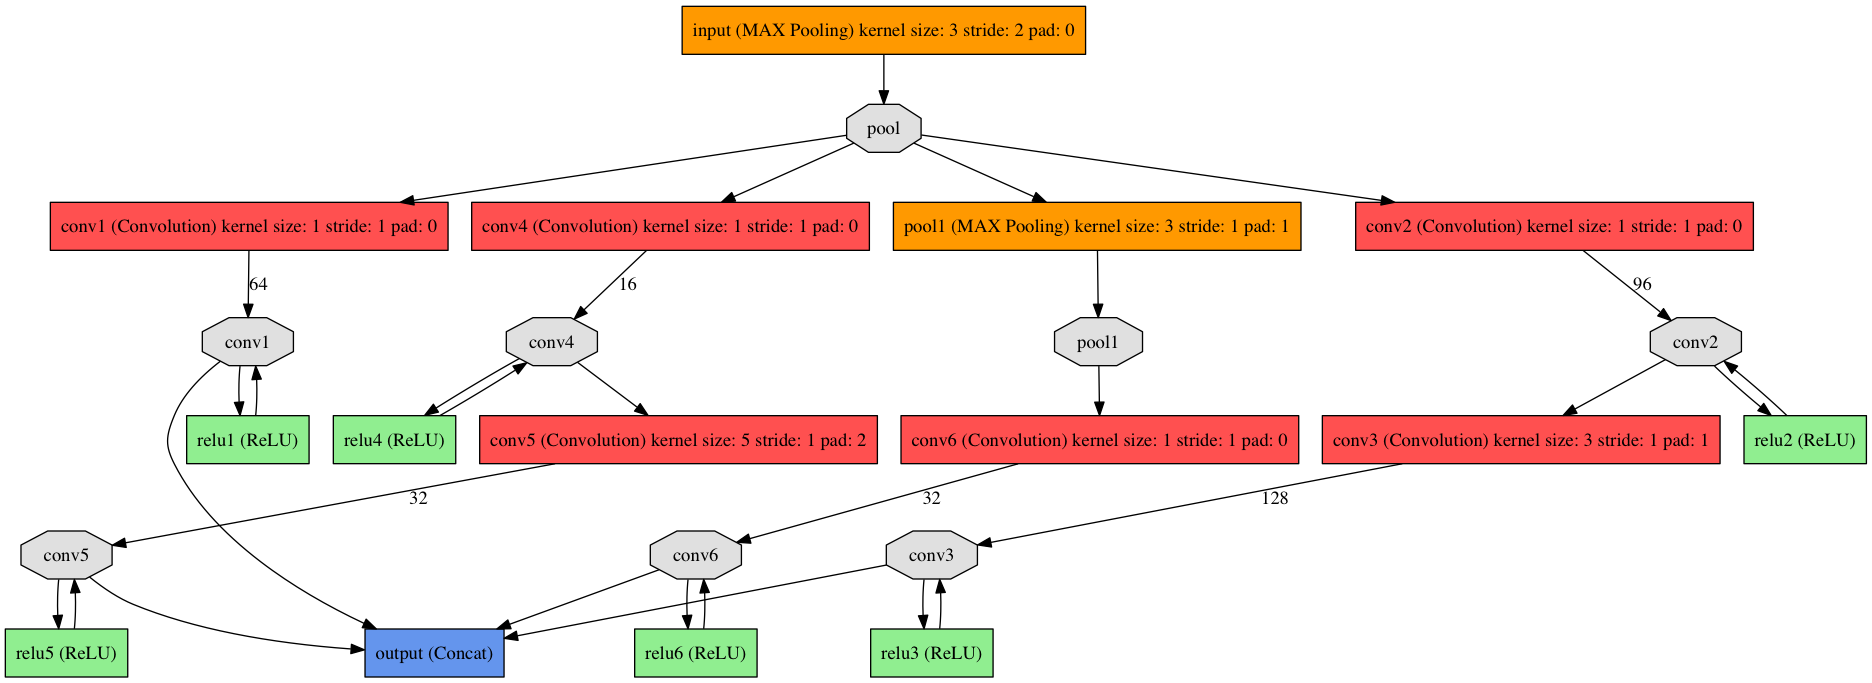
\includegraphics[width=0.95\textwidth]{figures/inception.png}
%  	\caption{Inception layer architecture}
%  	\label{fig:inception}
%\end{figure*} 

\section{Results and Discussion}
\label{sec:results_and_description}

We have experimented with both types of patches extraction and corresponding convolutional networks. 

\subsection{Deep convolutional network learning}

%\begin{figure}[!ht]
%\centering
%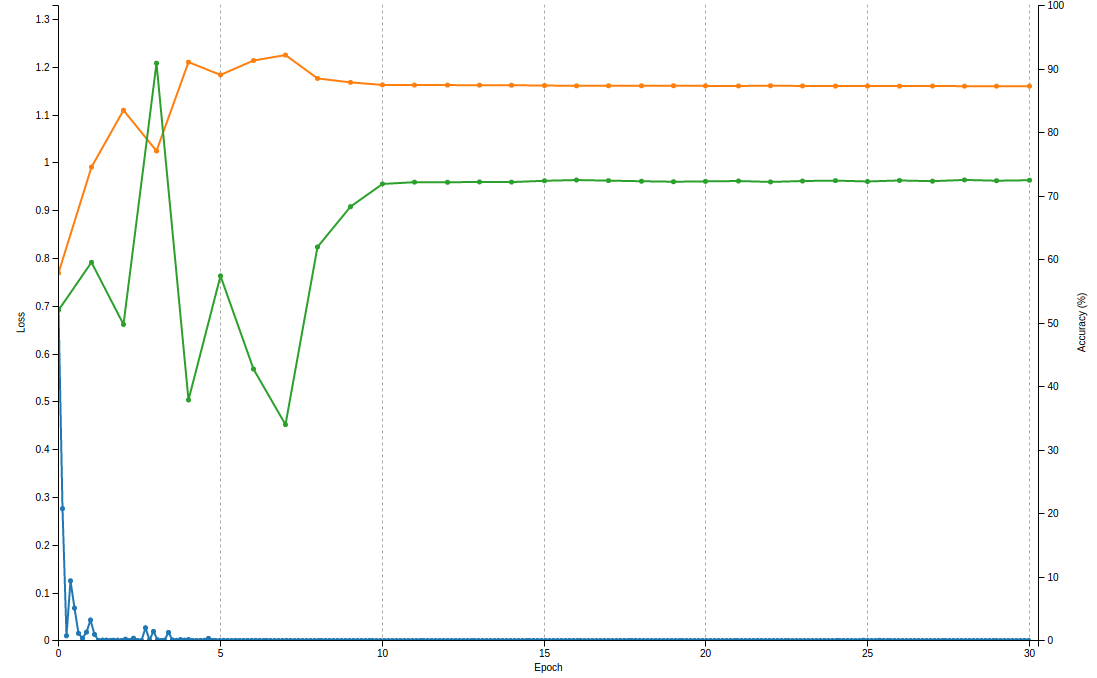
\includegraphics[scale=0.22]{figures/alexnet_loss.png}
%\caption{Sliding window patch convolution network learning process.}
%\label{img_alexnet}
%\end{figure}

Deep artificial networks have been trained with the backpropagation algorithm \cite{CNN} and shown small training error. For sliding window patch, convolution network accuracy value on the test set is near $87 \%$. For the connected components patch convolution network the accuracy is worse --- $80 \%$. 

During the training process deep convolutional network is trying to build a hierarchical structure of data presentation. On the first layers trained low-level features, on last layers -- some high-level representation of input data. This approach allows to build classifiers and successfully meet the challenges of supervised learning. To illustrate this idea, consider the feature activation of the first local response normalization layer (LRN) in the sliding window patch convolution network after feed forward through the network sliding window patch from Figure~\ref{fig:patches_example_sliding_window}. As can be seen in Figure~\ref{fig:lrn_activation} some feature maps are spiking at various Arabic words or combinations of words. This behavior demonstrates the purpose of this layer in the structure of the entire deep network.

In future studies it would be useful to use for training convolutional networks an additional training base such as KHATT \cite{khatt}.

\begin{figure}[!b]
	\centering
  	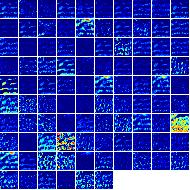
\includegraphics[width=0.75\linewidth]{figures/norm1.png}
	\caption{Features activations on the first local response normalization layer (LRN) in the sliding window patch convolution network.}
  	\label{fig:lrn_activation}
\end{figure}

\subsection{Manuscript classification}

To assess quality of the classification pipeline we have used only images from the test set, since they are the only ones not used in the learning process. 

Figure~\ref{fig:al_maqrizi_classification_example_train} demonstrates the classification results for two images from the test set: one from the al-Maqrizi class and one from the non-al-Maqrizi class. As one can see, both of them can be classified quite confidently as al-Maqrizi being the author with the probability $0.0085$ and $0.94$ respectively. Figure~\ref{fig:al_maqrizi_classification_example_test_hitat} shows the classification result for an {\it al-Khitat} manuscript page. It gives $0.77$ probability of al-Maqrizi being the author.

\begin{figure}[!t]
	\centering
  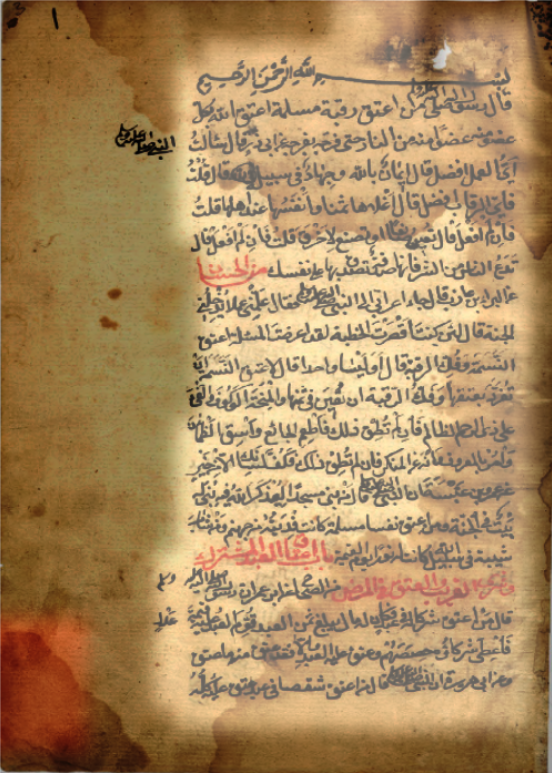
\includegraphics[width=0.49\linewidth]{figures/not_al_maqrizi_image_classification_example_fixed.png}
  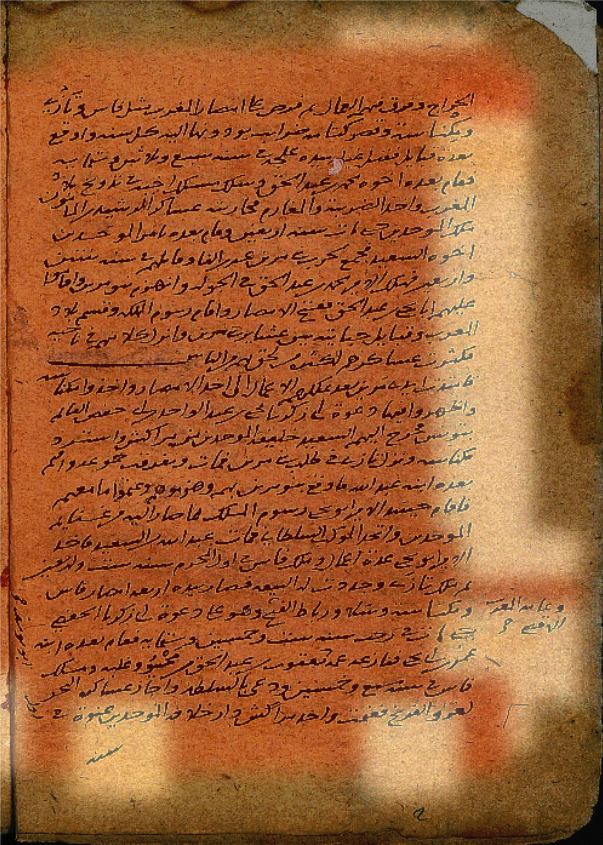
\includegraphics[width=0.49\linewidth]{figures/sw_al_maqrisi_fixed.png}
  \caption{Sliding window patches method of al-Maqrizi authorship classification example visualization. A non-al-Maqrizi manuscript page (left) and an al-Maqrizi manuscript page (right). Patches probabilities are visualized by using white-red colors (corresponding to 0-1 classes) on the top of the original image. The average al-Maqrizi authorship probability across patches is 0.0085 and 0.94 respectively.}
	\label{fig:al_maqrizi_classification_example_train}
\end{figure}

\begin{figure}[!t]
	\centering
  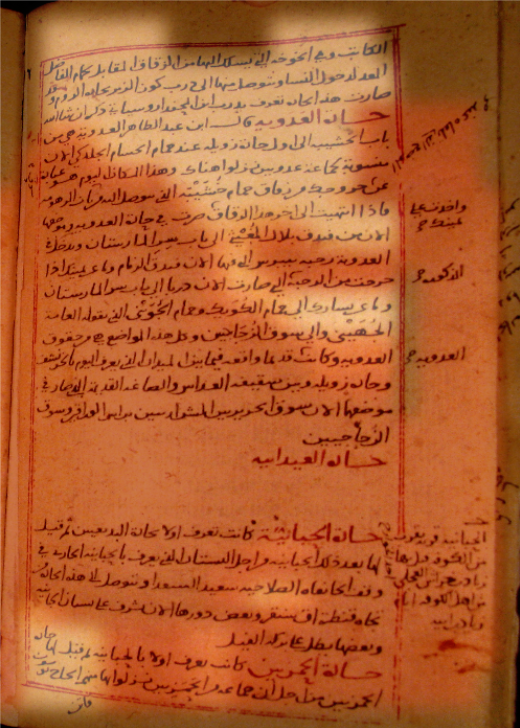
\includegraphics[width=0.49\linewidth]{figures/hitat_15_fixed.png}
   \caption{Sliding window patches method of al-Maqrizi authorship classification example visualization on the page from {\it al-Khitat} manuscript. On the average al-Maqrizi's authorship probability across the patches is 0.77.}
  %\captionof{figure}{ }
  %\label{fig:}
%  \captionof{figure}{Sliding window patches al-Maqrizi authorship classification example: %non-al-Maqrizi manuscript page (left), al-Maqrizi manuscript page (right) the transcript %page from {\it al-Khitat} (bottom). Patches probabilities are visualized by using white-%red colors (corresponding to 0-1 classes) on the top of the original image. Additionally, %a probabilities histogram is shown below.}
	\label{fig:al_maqrizi_classification_example_test_hitat}
\end{figure}

Regarding the entire test set classification for the sliding window patches with decision threshold $0.5$ we obtained the precision level of $0.99$ and recall $0.92$. The method, which based on connected components patches, is less robust: it generates many false positive predictions. This approach has a great potential, however, although its improvement requires many more training examples. In sum, convolutional network trained on connected components patches is a promising field for further research.

By using sliding window patches with the deep network method we have arrived at the conclusion that the mean probability of al-Maqrizi's authorship for the entire set of the {\it al-Khitat} pages equals $0.86$. 

In the future, the authors intend to implement the method of treating manuscript verification as the one-class classification problem.

\section{Conclusion}

The deep convolutional network with sliding window patches demonstrates very promising results in resolving the problem of the authorship of {\it al-Khitat}. In comparison with the other methods \cite{MBulacu}, \cite{MBulacu1}, \cite{DFecker}, \cite{Salvador} our approach shows a positive outcome without the need to construct complex features. To apply this method to other Arabic manuscripts, we will train our network on a larger volume of data. The joint study of al-Maqrizi's ``Description of Egypt'' undertaken by a historian-philologist and mathematicians is a unique experiment in working across disciplinary boundaries to achieve a common goal. The results obtained thus far bode well for the future by opening new horizons for scholars of ``Oriental'' manuscripts who often desperately lack resources (other than their own eyes and intuition) to verify the provenance and authorship of the manuscript material they are working with.

\section*{Acknowledgment}
The authors express their deep gratitude to Mrs. Evyn Kropf of the Hatcher Graduate Library who kindly facilitated access to the University of Michigan library resources.
 
 \begin{thebibliography}{1}

\bibitem{Noah} N.~Gardiner, F.~Bauden, \lq\lq A Recently Discovered Holograph Fair Copy of \textit{al-Mawa�iz wa-l-i�tibar fi dhikr al-khitat wa-al-athar} (Michigan Islamic MS 605),\rq\rq~in~\emph{Journal of Islamic Manuscripts}, vol.~2, E.~J.~Brill, Leiden and Boston, 2011, pp.~123--131.

\bibitem{MBulacu} M.~Bulacu, L.~Schomaker, A.~Brink, \lq\lq Text-independent Writer Identification and Verification on offline Arabic Handwriting,\rq\rq~in~\emph{Proc. 9th International Conference on Document Analysis and Recognition, ICDAR}, Curitiba, 2007, pp.~769--773.

\bibitem{MBulacu1} M.~Bulacu, L.~Schomaker, \lq\lq Automatic Handwriting Identification on Medieval Documents,\rq\rq~in~\emph{Proc. of the International Conference on Image Analysis and Processing}, Modena, 2007, pp.~279--284.

\bibitem{DFecker} D.~Fecker, A.~Asi, W.~Pantke, V.~Margner, J.~El-Sana, T.~Fingscheidt, \lq\lq Document Writer Analysis with Rejection for Historical Arabic Manuscripts,\rq\rq~in~\emph{Proc. 14th International Conference on Frontiers in Handwriting Recognition, ICFHR}, Crete, 2014, pp.~743--748.

\bibitem{Salvador} S.~Godoy-Calderon, E.~M.~Felipe-Riveron, E.~C.~Herrera-Luna, \lq\lq Multi-level Modeling of Manuscripts for Authorship Identification with Collective Decision Systems,\rq\rq~\emph{Progress in Pattern Recognition, Image Analysis, Computer Vision, and Applications}, vol.~7441, pp.~757--764, 2012.

\bibitem{Dunn} E.~Dunn, \lq\lq Computational Methods for Determining the Similarity between Ancient Greek Manuscripts,\rq\rq~Master of Science~thesis, Dept.~Computer~Science., Dept.~Inform.~Systems~and~Operations~Manag. Univ.~of North Carolina, Wilmington, 2012.

\bibitem{DL} Y.~Lecun, Y.~Bengio, G.~Hinton, \lq\lq Deep learning,\rq\rq~\emph{Nature}, no.~521, pp.~436--444, May.~2015.

\bibitem{CNN} Y.~Lecun, L.~Bottou, Y.~Bengio, P.~Haffner, \lq\lq Gradient-based learning applied to document recognition,\rq\rq~in~\emph{Proc. of the IEEE}, 1998, pp.~2278--2324.

\bibitem{DL_Arabic_1} S.~Yousfi, S.-A.~Berrani, C.~Garcia, \lq\lq Deep learning and recurrent connectionist-based approaches for Arabic text recognition in videos,\rq\rq~in~\emph{Proc. of the 13th International Conference on Document Analysis and Recognition (ICDAR)}, 2015, pp.~1026--1030

\bibitem{DL_Arabic_2} W.~Yang, L.~Jin, M.~Liu, \lq\lq Character-level Chinese Writer Identification using Path Signature Feature, DropStroke and Deep CNN,\rq\rq~in~\emph{Proc. of the 13th International Conference on Document Analysis and Recognition (ICDAR)}, 2015, pp.~546--550

\bibitem{Alexnet} A.~Krizhevsky,I.~Sutskever, G.~Hinton, \lq\lq ImageNet Classification with Deep Convolutional Neural Networks,\rq\rq~in~\emph{Advances in Neural Information Processing Systems}, vol.~25, 2012, pp.~1097--1105.

\bibitem{Googlenet} C.~Szegedy, W.~Liu, Y.~Jia, P.~Sermanet, S.~Reed, D.~Anguelov, D.~Erhan, V.~Vanhoucke, A.~Rabinovich, \lq\lq Going deeper with convolutions,\rq\rq~in~\emph{Proc. of the IEEE Conference on Computer Vision and Pattern Recognition}, Boston, 2015, pp.~1--9.

\bibitem{otsu1975threshold} N.~Otsu, \lq\lq A threshold selection method from gray-level histograms, \rq\rq~\emph{Automatica}, vol.~11, 1975, pp.~285--296.

\bibitem{fiorio1996connected_components} C.~Fiorio, J.~Gustedt, \lq\lq Two linear time union-find strategies for image processing, \rq\rq~\emph{Theoretical Computer Science}, vol.~154, no.~2, 1996, pp.~165--181.

\bibitem{ester1996dbscan} M.~Ester, H.P.~Kriegel, J.~Sander, X.~Xu, \lq\lq A density-based algorithm for discovering clusters in large spatial databases with noise, \rq\rq~in~\emph{Proc. of Second International
Conference on Knowledge Discovery and Data Mining}, vol.~96, no.~34, 1996, pp.~226--231.

\bibitem{GranVolk} O.~Granichin, V.~Volkovich, D.~Toledano-Kitai, \emph{Randomized Algorithms in Automatic Control and Data Mining}. Springer-Verlag: Heidelberg, New York, Dordrecht, London, 2015, 251~p.

\bibitem{khatt} S.~A.~Mahmoud, I.~Ahmad, M.~Alshayeb, W.~G.~Al-Khatib, M.~T.~Parvez, G.~A.~Fink, V.~Margner, H.~El Abed, \lq\lq KHATT: Arabic offline handwritten text database, \rq\rq~in~\em{ Proc.13th International Conference on Frontiers in Handwriting Recognition (ICFHR)}, 2012, pp.~447--452.

\end{thebibliography}

\end{document}
